%!TEX root = ../projecto.tex
\section{Related Work} % (fold)
\label{sec:related_work}

This section provides insight of work done in multiple research areas that are related to the project. In subsection \ref{sub:self_organizing_maps} will be described multiple work done using Self-organizing maps. Subsection \ref{sub:topic_detection_on_twitter} is dedicated to work done on topic detection on the social network Twitter \footnote{http://www.twitter.com}

\subsection{Self-organizing Maps} % (fold)
\label{sub:self_organizing_maps}
Self-organizing maps are used in a wide are of applications, from authentications systems \cite{Dozono2012}, network intrusion detection \cite{intrusion_som} and speech recognition and analysis \cite{phonetic_typewiter}.

\subsubsection{Detecting Hidden Patterns on Twitter Usage} % (fold)
\label{ssub:detecting_hidden_patterns_on_twitter_usage}

\citep{Cheong2010} analyzed hidden patterns created buy the natural usage of twitter by its users. In its study they started by collecting dallta from the twitter API different kinds of topics like "2009 Iran Election" and "iPhone 3.0 OS launch". They made multi level signal extraction not only from information directly present on the tweet, but also by cross referencing with other social website and with the twitter user profile information. The signals retrieved from the social network can be seen in table \ref{tab:twitter_signals}.

\begin{table}[H]
  \caption{Twitter Signals}
  \label{tab:twitter_signals}
  \begin{center}
    \begin{tabular}{|l|l|l|}
    \hline

    \hline
    \textbf{Twitt Corpus} & \textbf{Twitter Profile} & \textbf{External Sources} \\
    \hline
       Tweet Size & Gender & Other Social Network Accounts\\
    \hline
       Replies & Number of customizations & Type of website\\
    \hline
       Re-tweets & Friends to followers ratio & \\
    \hline
       Hashtags & frequency of posts & \\
    \hline
      \specialcell{Presence of URIs and \\ Type of linked content}
        & Account Age
        & \\
    \hline
       Type of Device & Country & \\
    \hline
       Tweet Location &  & \\
    \hline
    \end{tabular}
  \end{center}
\end{table}

By applying clustering algorithm of SOM, they could find 4 demographical clusters during the Iran 2009 Election. The first cluster was characterized by young web-based Iranians, with twitter accounts not older than 3 months with a high frequency of replies. The second cluster was mainly compound of web users from Iran accounts older that 3 months. The third cluster had Iranian users with mobile clients with large texts clearly trying to raise awareness. The fourth and final cluster represented the users around the world trying to raise awareness about the issue by sharing tweets with URIs.
Looking at their analysis about the topic "2009 Iranian Election" it is clear to see that it was possible to describe the type of users represented in the social network and the way they interact with it.

On the iPhone 3.0 OS launch it was possible to find three main clusters. The first cluster was characterized by male users, accounts older than 90 days, coming from countries where the iPhone is marketed, with high adoption of social media clearly representing the target market of the iPhone or its customers. The second cluster had new accounts with higher rate of followers to followees, high frequency of posts per day, presence of URI linking to technology blogs or websites, no country or gender specified meaning that this cluster was clearly composed by news aggregators and technological news websites. Inside the second cluster there was a sub-cluster of Japanese users which represents the high rate of iPhone adoption in Japan. Finally the third cluster was clearly spammer accounts that where eventually deleted after a couple of months, characterized by popular social connections, posting more than 50 tweets a day with external URIs and the accounts where not older than a day or so.

In conclusion it was possible to detect Twitter usage patterns and specifically detect spammers before they where banned from the social network. 
% subsubsection detecting_hidden_patterns_on_twitter_usage (end)

\subsubsection{Types of SOMs} % (fold)
\label{ssub:types_of_soms}

Depending on the kind of data that scientist are trying to analyze and visualize, different approaches can be made the SOM algorithm in order to better adapt to the data at hand.

Weight adaptation SOMs are simple Self-organizing maps in which the weights of the vector space model are not even. For example \citet{Bacao2005}  proposed the adaptation of the algorithm in order to better represent geographical data where more weight is given to the coordinates of the data.

First introduced by \citet{multi_layer_semantics}, the Hierarchical SOMs are often used when it is possible to decompose on big problem into smaller problems. One or more SOMs are located at each layer usually operating in on different variables. The hierarchical SOM allows the creation of thematic classifications at lower layers which are then composed into a single one \citet{Bacao2005} which leads to a more specific kind of classification in the lower layers. 
Based on the survey made by their work \citet{Henriques2012} suggests that there are four main types of hierarchical SOMs, Thematic Agglomerative, Agglomerative HSOM based on clusters, static devised HSOM and dynamic devised HSOM.
Multi layered SOMs where used by \citet{Rauber2000} on automatically detect and organize topics in order to organize bookshelves. They used the vector space model to define all books and started initially with only four cluster, that where consequently sub-divided and categorized which in the end created a hierarchical tree of topics.
Multi layered SOMs have been used in a wide variety of applications, such as speech recognition \citet{multi_layer_semantics} and learning to control a robot arm and wrist \citet{Sayers1991}.


The Geo-SOM \citet{Bacao2005} applies the first law of geography “Everything is related to everything else, but near things are more related than distant things." to the SOM algorithm, where the winning neuron is chosen by in a radius k defined by the geo-coordinates of the data. In this way the Geo-som forces units that are close in the input space to be close in the output space. The representation of the Geo-som can be seen in figure \ref{fig:geo_som}.



\begin{figure}[tb]
  \begin{center}
    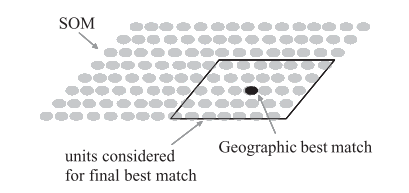
\includegraphics[]{images/6_geo-som.png}
  \end{center}
  \caption{Geo-SOM structure, from \citet{Bacao2005}}
  \label{fig:geo_som}
\end{figure}


Self organizing maps have their own limitations mainly drawing from the fact that it has a fixed number of neurons. \citet{Qiang2010} cites in his survey about the state of self organizing maps, that newer algorithms namely Growing cell Structures \cite{Fritzke1995} and Growing Neural Gas \cite{Fritzke1994} don't have this drawback.
% subsubsection types_of_soms (end)

% subsection self_organizing_maps (end)


\subsection{Topic Detection and Clustering} % (fold)
\label{sub:topic_detection_on_twitter}
There have been many topic detection techniques used throughout the time. Many of them rely on the TF IDF (term frequency – inverse document frequency, based on IDF by \citet{Jones2004}) which is not particularly adequate for topic detection on Twitter due to the fact that tweets are very small, composed by typos or slang words and might be written in multiple languages, sometimes at the same time. In this subsection we will take a look at multiple methods of topic detection in general and specifically on the Twitter social network.

\subsubsection{Topic and Trending Detection} % (fold)
\label{ssub:real_time_topic_and_trending_detection}
Due to the social rapid social adaptation from people to always be on-line, through the usage of cellphones on the move desktops at work and even TV at home, the increase of user generated content has increased tremendously in latest years. In 2006 35"\%" of on-line adults and 57"\%" of teenagers created content on the Internet \footnote{ Data source: http://www.pewinternet.org/Presentations/2006/UserGenerated-Content.aspx} which in "Internet Years" was ages ago.
With amount of content increasing, new real-time and scalable algorithms are needed in order to make sense of all this data.
\citet{Cataldi2010} proposes a new technique for emerging topic detection that permits real-time retrieval of the most emergent topics expressed by a community on Twitter. Their work applies the PageRank \cite{Pagerank1998} algorithm to the users follower / followee relationship in order to find the most influential user on the network and then calculate the more trending topics by relating, social influence, word co-occurrence and time frame. In the end an interface was created where it would be possible to navigate hot topics in a given time frame. It is important to say that topic labeling was not automatic and was implicit by the time frame of an event, if two highly social events would occur in the same time frame with word relations the results could be interpreted as the same, for example if a political candidate would win the elections at the same of an important sport club would win it specific cup, the word win could be trending at the same time for two different topics and due to high temporal dependency they could be interpreted as the same topic.
\citet{Weng2010} also used the PageRank algorithm in order to find the most influential twitter users on a certain topic, but uses a different approach where they represent each twitter user as a bag of words comprising of all the tweets that they have posted, afterwards it uses Latent Dirichlet Allocation \cite{Blei2003} in order to find the topics each user is interested in. In the end it was possible to prove that follower / followee relation on twitter was not just casual, but that people actually follow other people in which they have some resemblance or common interest, this concept is called homophily and will be further explored by this project.

\citet{Sudhof2011} presents a model to where for a given user and a certain topic, it can evaluate the user side on a determined manner of case. For example 

\subsection{Data Mining in Twitter } % (fold)
\label{sub:data_mining_in_twitter_}
In this subsection, we will focus on work done on Twitter social network in order to leverage insights on how the public data available from the website can correlated within itself and with outside sources. 

\subsubsection{Enhancing the Tweet} % (fold)
\label{ssub:the_tweet}
Tweet retrieval and analysis is a double edged problem. On one side the tweet is really small which makes it almost impossible to retrieve any actual sense from it. On the other hand the amount of tweets generated per day is around 140 million \footnote{https://blog.twitter.com/2011/numbers} wich means that it is very hard to to deep analyses the semantics and content of individual tweets, but if so is done, only the more appropriate signals should be evaluated.
\citet{Tao2012} evaluated how the multiple signals that could be retrieved directly or indirectly from the tweet corpus could mean that a tweet is relevant for a determined topic. In his work, Tao presents premises that seem intuitively true and proves if they actually are relevant through comparison of multiple precision and recall values. Its results on feature comparison where summarized in table \ref{tab:tao_table}, the first row consists of all the made hypothesis categorized by type, and the second row tells if the data used actually influenced in precision and recall results.

\begin{table}[tb]
  \caption{\citet{Tao2012} resumed results}
  \label{tab:tao_table}
  \begin{tabularx}{\textwidth}{|X|l|}
  \hline
  \textbf{Hypotheses} & \textbf{Influence of Features} \\
  \hline
  \hline

  {\bf Syntatical} &  \\
  \hline
  Tweets that contain Hashtags are more likely to be relevant than tweets that don't & Not Important \\
  \hline
  Tweets that contain an URI are more relevant that tweets that don't  &Important \\
  \hline
  Tweets that are replies to other tweets are less relevant & Important \\
  \hline
  The longer the tweet is the more relevant it is & Not Important\\
  \hline
  \hline

  {\bf Semantic}  &  \\
  \hline
  
  The more the number of entities the more relevant a tweet is  & Important \\
  \hline
  Different types of entities are of can have different amount of interest to a give topic  & Important \\
  \hline
  The greater the diversity of concepts mentions in a tweet the more likely for it to be relevant & Important \\
  \hline
  The relevance of a tweet is determined buy its polarity & Important \\
  \hline
  \hline

  {\bf Contextual} &  \\
  \hline
  The lower the temporal distance between a query and the creation of a tweet the more relevant the tweet is  & Not Important \\
  \hline
  The more the number of tweets created by a user the more relevant one of his tweets will be & Not Important \\
  \hline
  \end{tabularx}
\end{table}

Tau also compared result of topic characteristics, concluding that distinction between local and global events as well as temporal persistence proved to not be relevant on relevance prediction.

\citet{McCreadie2013} also approached the issue of having very little content on tweets in order to categorize a tweet, and tried to solve it by applying the content of linked URIs into the tweet body in order to improve precision and recall. The best fitting approach was using Field-Based weighting where for each tweet a new document is created which contains two fields; the terms in the tweet and the terms in the linked document. 
Afterwards a learning to rank algorithm PL2F is used against the dataset from Microblog2011 in order to find the best weighting that should be applied to the tweet corpus and the URI referenced page. 
With this trained model they where able to improve precision in an order of 0.9. 

\subsubsection{Rapidly Changing Trends} % (fold)
\label{ssub:real_time_}
Due to the real time nature of Twitter, using typical retrieval model that rely on term frequency models like BM25 or language modeling cannot be applied as stated by \citet{Lin2012}. The study of topic perdurance on the social network proved that it is presented in bursts of queries and mentions of a topic. The typical usage of twitterr for search is not the same of Google, when user are searching in twitter they want to find out what is happening right know meaning that classification techniques based on past events cannot respond this kind problem. As stated by \citet{Lin2012} this problem has not yet been solved at twitter (or anywhere else at the time of writing this report), and issues a new kind of data analysis approach that was not taken into consideration in the past. 
This effect of rapidly changing topics and queries based on real time events was named "Churn", and can be clearly seen in figure \ref{fig:churn}.

  \begin{figure}[tb]
    \begin{center}
    \noindent\makebox[\textwidth]{
      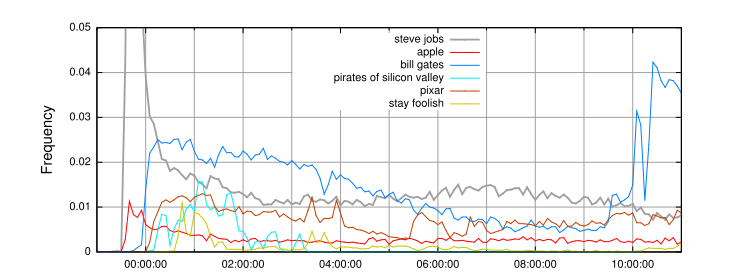
\includegraphics[width=13cm]{images/7_churn.png}
    }
    \end{center}
    \caption{The Churn effect: Frequencies of queries related to Steve Jobs death over a 12 hour period in 5-minute intervals, normalized to the total number of queries in the interval. At its peak, the query “steve jobs” reaches 0.15 (15\% of the query stream); Graph taken from \cite{Lin2012}}
    \label{fig:churn}
  \end{figure}

% subsubsection real_time_ (end)
% subsubsection the_tweet (end)
% subsection data_mining_in_twitter_ (end)
% subsubsection real_time_topic_and_trending_detection (end)
% subsection topic_detection_on_twitter (end)
% section related_work (end)
